\documentclass[a4paper, 11pt, oneside]{report} 

\usepackage{graphicx}
\usepackage{float}
\usepackage[dvipsnames,table,xcdraw]{xcolor}
\usepackage[utf8]{inputenc} 
\usepackage[T1]{fontenc} 
\usepackage{amsmath}
\usepackage{amssymb}
\usepackage{amsfonts} 
\usepackage{subcaption}
\usepackage{tikz}
\usetikzlibrary{shapes,positioning,fit,calc,backgrounds}
\usepackage{pgfplots}
\pgfplotsset{compat=1.18}
\usepackage{longtable}
\usepackage{booktabs}
\usepackage{array}
\usepackage[nottoc]{tocbibind}
\usepackage{url}
\usepackage{hyperref}
\usepackage{amsmath}

\hypersetup{
    colorlinks=true,
    linkcolor=blue!80!black,
    citecolor=green!60!black,
    urlcolor=blue!70!black
}

\begin{document} 	

	\begin{titlepage} 
		\centering 
		\vspace*{\baselineskip} 
		\vspace{0.75\baselineskip}
		
		{\LARGE \textbf{OpsMind AI: Enterprise Standard Operating Procedure (SOP) Knowledge Assistant with Retrieval-Augmented Generation}}
		
		\vspace{1.5\baselineskip}

		An internship report submitted for the course named\\
		\textbf{Internship (CS4XX)}
		
		\vspace*{4\baselineskip}
		
		Submitted By
		
		\vspace{0.5\baselineskip}
		
		{\scshape\Large Krishna Anand\\ SEMESTER - VII \\ Roll No: 230101082}
		
		\vspace{1.5\baselineskip}
		
		Under the Guidance of
		
		\vspace{0.5\baselineskip}
		
		{\scshape\Large Dr. Rajkumari Bidyalakshmi Devi\\ Department of Computer Science and Engineering}
		
		\vfill
		
		\begin{center}
			
\includegraphics[width=4.5cm]{report_file/iiit manipur.png}
		\end{center}
	
	{\scshape\small Department of Computer Science and Engineering\\ Indian Institute of Information Technology Senapati, Manipur \\ Month, Year}
	
\end{titlepage}

%----------------------------------------------------------------------------------------
% Declaration
%----------------------------------------------------------------------------------------

\newpage
\begin{center}
   { \LARGE \textbf{Declaration}}
\end{center}
\vspace{1cm}
In this submission, I have expressed my idea in my own words, and I have adequately cited and referenced any ideas or words that were taken from another source. I also declare that I adhere to all principles of academic honesty and integrity and that I have not misrepresented or falsified any ideas, data, facts, or sources in this submission. If any violation of the above is made, I understand that the institute may take disciplinary action. Such a violation may also engender disciplinary action from the sources which were not properly cited or permission not taken when needed.

\vspace{2cm}
\begin{flushright}
KRISHNA ANAND \\
Roll No: 230101082 \\
Date: \today
\end{flushright}

%----------------------------------------------------------------------------------------
% Certificate
%----------------------------------------------------------------------------------------

\newpage
\thispagestyle{empty}
\begin{center}
	\begin{table}[H]
		\centering
		
\includegraphics[scale=0.18]{report_file/iiit manipur.png}
		\begin{tabular}{l}
			\textbf{Department of Computer Science and Engineering} \\
			\textbf{Indian Institute of Information Technology Senapati, Manipur} \\
		\end{tabular}
	\end{table}
	\par\noindent\rule{\textwidth}{0.4pt}
	\vspace{0.3cm}
	
	\begin{flushleft}
	Dr. Rajkumari Bidyalakshmi Devi \hfill Email: \href{mailto:bidyalakshmi@iiitmanipur.ac.in}{bidyalakshmi@iiitmanipur.ac.in}\\
	Assistant Professor \hfill Contact No: +91-7005126046\\
	\end{flushleft}
	
	\vspace{0.6cm}
	{\LARGE \textbf{\emph{To Whom It May Concern}}}\\[0.8cm]
	\linespread{1.2}
	\large{This is to certify that the internship report entitled \textbf{``OpsMind AI: Enterprise Standard Operating Procedure (SOP) Knowledge Assistant with Retrieval-Augmented Generation'',} submitted to the Department of Computer Science and Engineering, Indian Institute of Information Technology Senapati, Manipur in partial fulfillment for the award of degree of \textbf{Bachelor of Technology in Computer Science and Engineering} is a record of bonafide work carried out by \textbf{Krishna Anand} bearing roll number \textbf{230101082}.}\\[1.2cm]
	
	\begin{flushright}
	\large{Signature of Faculty Advisor}\\[0.3cm]
	\textbf{(Dr. Rajkumari Bidyalakshmi Devi)}\\[0.3cm]
	\end{flushright}
		
\end{center}
\vspace{0.4cm}
\noindent Signature of the Examiner 1: ....................................................\\[0.5cm]
\noindent Signature of the Examiner 2: ....................................................\\[0.5cm]
\noindent Signature of the Examiner 3: ....................................................\\[0.5cm]
\noindent Signature of the Examiner 4: ....................................................

%----------------------------------------------------------------------------------------
% Internship Documents Notice
%----------------------------------------------------------------------------------------

\newpage
\begin{center}
    {\LARGE \textbf{Internship Documents}}
\end{center}
\vspace{1cm}
\textbf{Attach Internship Offer Letter(s) and Internship Completion Certificate(s) here.}

\vspace{1cm}
\textbf{Report}: At the end of the internship, students need to submit a comprehensive internship report duly signed by the supervisor/mentor appointed by the industry/institute to the Head of Department along with the internship offer-letter. In case of multiple internships, multiple offer letters must be submitted. The internship report must include a certificate from the supervisor stating that the work done is genuine and is not copied from any other sources. The name of the supervisor, designation, name of the organization, official email ID, and phone number should be clearly stated.

\vspace{1cm}
\textbf{Evaluation}: Students need to present the work done to the evaluation committee of the CSE department, IIIT Manipur.

%----------------------------------------------------------------------------------------
% Abstract
%----------------------------------------------------------------------------------------

\newpage
\begin{abstract}
In large-scale enterprise environments such as automated fulfillment centers, logistics hubs, and regulatory compliance units, Standard Operating Procedures (SOPs) are critical for ensuring operational fidelity, safety adherence, and procedural compliance. However, employees frequently encounter significant operational latency and cognitive friction when navigating multi-hundred-page technical PDF documentation. Traditional keyword-based retrieval methods (e.g., BM25) fail to resolve semantic paraphrasing and conceptual intent, while raw generative Large Language Models (LLMs) present substantial compliance risks due to their susceptibility to hallucinations and lack of verifiable provenance.

To address these challenges, this report presents \textbf{OpsMind AI}, an enterprise-grade SOP Knowledge Assistant based on the paradigm of Retrieval-Augmented Generation (RAG). OpsMind AI automates the end-to-end ingestion and indexing of complex PDF manuals by executing text stream parsing, sliding-window chunk segmentation ($1,000$ characters with $100$ character overlap), domain section categorization, and in-process dense vector generation using the 384-dimensional \texttt{all-MiniLM-L6-v2} Transformer model. High-dimensional vector representations are indexed directly within MongoDB Atlas, enabling sub-second Approximate Nearest Neighbor (ANN) cosine similarity retrieval.

Upon receiving a natural language query, the system retrieves the top-$k$ most relevant context segments, validates relevance against a strict similarity threshold ($\tau = 0.65$), and synthesizes a factually grounded response using Google Gemini 2.5 Flash. Every answer is coupled with granular source attribution—including document name, exact page number, section category, chunk index, and cosine similarity score—with interactive modal snippet verification. Empirical evaluation on an enterprise SOP manual of 46 pages and 205 indexed chunks demonstrated an end-to-end response time of $865\text{ ms}$, $100\%$ grounding accuracy on verified procedures, and zero hallucination on out-of-domain inquiries.
\end{abstract}

%----------------------------------------------------------------------------------------
% Acknowledgement
%----------------------------------------------------------------------------------------

\newpage
\begin{center}
    { \LARGE \textbf{Acknowledgement}}
\end{center}
\vspace{1.5cm}
I would like to express my sincere gratitude and deep respect to my faculty advisor, \textbf{Dr. Rajkumari Bidyalakshmi Devi}, Department of Computer Science and Engineering, Indian Institute of Information Technology Senapati, Manipur, for providing invaluable guidance, constructive feedback, and continuous support throughout the duration of this internship.

I extend my heartfelt thanks to the Head of the Department and the esteemed faculty members of the Department of Computer Science and Engineering, IIIT Manipur, for providing the necessary academic infrastructure, computational resources, and encouraging environment essential for the completion of this work.

I am also thankful to my peers, friends, and family for their unwavering encouragement, insightful discussions, and moral support during the design, implementation, and documentation of OpsMind AI.

\vspace{2cm}
\begin{flushright}
Krishna Anand\\
Roll No: 230101082\\
Department of Computer Science and Engineering\\
Indian Institute of Information Technology Senapati, Manipur
\end{flushright}

%----------------------------------------------------------------------------------------
% Table of Contents, Lists
%----------------------------------------------------------------------------------------

\newpage
\tableofcontents
\listoffigures
\listoftables

%----------------------------------------------------------------------------------------
% Main Chapters
%----------------------------------------------------------------------------------------

\chapter{Introduction}
\section{Outline}
\label{sec:intro_outline}

In modern distributed enterprise environments, organizational knowledge is heavily codified into formal operational guidelines known as Standard Operating Procedures (SOPs). These documents define baseline standards, compliance mandates, troubleshooting workflows, incident response protocols, logistics guidelines, and administrative hierarchies across departments. As enterprises expand their operational footprint, SOP repositories scale rapidly in volume, complexity, and domain specialization. 

Traditional information management systems typically rely on manual folder structures, intranet portals, and static keyword indexing techniques (such as boolean string matching or BM25 probabilistic ranking). In high-throughput industrial settings—such as automated fulfillment centers, supply chain delivery hubs, cross-docking warehouses, customer support centers, and regulated compliance offices—personnel encounter severe cognitive friction when attempting to locate granular, unambiguous answers within dense, multi-hundred-page technical manuals. 

The advent of Large Language Models (LLMs) and Transformer-based natural language processing has introduced transformative possibilities for conversational knowledge access. However, deploying raw generative models directly in enterprise knowledge workflows introduces severe risks, most notably \emph{hallucination} (the generation of factually unsupported or fabricated statements), lack of verifiable source provenance, and an inability to dynamically integrate proprietary, internal documentation without costly fine-tuning.

To solve these systemic bottlenecks, this internship develops \textbf{OpsMind AI}, an intelligent, enterprise-grade SOP Knowledge Assistant built upon the paradigm of \emph{Retrieval-Augmented Generation} (RAG). OpsMind AI ingests unformatted organizational SOP documents in Portable Document Format (PDF), parses and segments dense content into overlapping semantic text chunks, projects these textual representations into a high-dimensional continuous metric space using dense transformer embeddings, indexes them within a cloud-native vector database, and executes semantic vector retrieval to feed context-bounded prompts into Google's state-of-the-art Gemini Large Language Model. The system strictly enforces attribution, displaying the exact source document, page number, operational section header, chunk identifier, and cosine similarity metric alongside every synthesized answer.

\section{Problem Statement}
\label{sec:intro_problem_statement}

Enterprise knowledge retrieval within operational environments faces several critical challenges:

\begin{enumerate}
    \item \textbf{High Information Latency and Operational Friction:} Employees, floor leads, and administrative personnel spend disproportionate time manually searching through voluminous PDFs to find specific guidelines (e.g., Return-to-Stock target rates, parcel weight tolerances, hazard containment procedures, or escalation matrices). This manual lookup increases task completion time and degrades frontline productivity.
    \item \textbf{Limitations of Lexical Search:} Traditional keyword-based search algorithms fail when the user's query vocabulary diverges from the exact phrasing in the source manual. Conceptual inquiries (e.g., asking about ``workflow for handling damaged goods'' versus manual headings stating ``Damaged Inventory Processing'') yield poor recall or irrelevant matches.
    \item \textbf{Hallucination and Compliance Vulnerability in Standard AI Models:} Generic generative AI systems answer queries based on parametric knowledge acquired during pre-training. In enterprise contexts, parametric guessing can lead to severe operational errors, safety violations, or compliance breaches. A dependable enterprise system must provide strictly grounded answers and explicitly decline to answer when the information is absent from authorized documentation.
    \item \textbf{Absence of Granular Source Attribution:} Standard conversational agents provide text responses without traceable evidence. Without instant visibility into the exact originating page, document name, and text excerpt, human operators cannot independently audit or verify AI-generated answers.
\end{enumerate}

\section{Motivation}
\label{sec:intro_motivation}

The primary motivation behind OpsMind AI is to bridge the operational gap between static enterprise documentation and agile human decision-making. By converting static PDF manuals into an interactive, semantic knowledge graph, organizations can democratize access to critical operating knowledge while maintaining mathematical precision, complete auditability, and zero tolerance for fabricated answers.

Modern fulfillment centers, delivery hubs, and administrative divisions require sub-second access to operational parameters. When an operator queries an approval chain, a cycle count frequency, or an emergency evacuation protocol, the assistant must return not only the definitive procedure but also the exact page reference for institutional accountability. 

Furthermore, building an end-to-end decoupled architecture—integrating in-process dense embedding pipelines, scalable vector database indexing, and advanced generative reasoning—provides a cost-effective, maintainable blueprint for next-generation enterprise knowledge management without requiring massive model retraining or specialized hardware clusters.

\section{Purpose}
\label{sec:intro_purpose}

The purpose of this internship work is to design, implement, and rigorously evaluate an end-to-end enterprise knowledge retrieval and conversational assistant system. Specifically, the internship aims to fulfill the following objectives:

\begin{itemize}
    \item \textbf{Automated Document Ingestion and Segmentation:} Develop an automated ingestion pipeline capable of parsing multi-page enterprise PDF documents, executing intelligent text extraction, and generating normalized, overlapping text chunks to preserve local context across boundaries.
    \item \textbf{Domain-Specific Section Categorization:} Implement an automated heuristic classification system that identifies operational sections (e.g., Inbound Operations, Inventory Audit Framework, Outbound Operations, Safety, Business Continuity) and attaches rich metadata to segmented chunks.
    \item \textbf{Dense Semantic Vector Generation:} Integrate high-efficiency transformer embeddings via in-process neural pipeline architectures (utilizing the 384-dimensional \emph{all-MiniLM-L6-v2} model) to capture deep semantic relationships between operational queries and document segments.
    \item \textbf{Scalable Vector Indexing and Similarity Search:} Deploy and configure a high-dimensional vector search index within MongoDB Atlas, enabling sub-second approximate nearest neighbor (ANN) retrieval with cosine similarity scoring.
    \item \textbf{Strictly Grounded Generative Synthesis:} Integrate Google's Gemini 2.5 Flash generative model through structured, zero-hallucination prompt constraints, enforcing that all answers are synthesized strictly from retrieved contextual snippets with a conservative similarity threshold fallback mechanism.
    \item \textbf{Interactive User and Administrative Interfaces:} Construct a responsive, modern web interface with dual-theme capabilities, real-time citation viewing with modal snippet inspection, dynamic document analytics, and administrative document lifecycle management.
\end{itemize}


\chapter{Literature Survey}
\section{Evolution of Enterprise Information Retrieval}
\label{sec:lit_ir_evolution}

Information Retrieval (IR) in organizational contexts has evolved across three distinct generations: classical lexical matching, dense vector semantic retrieval, and retrieval-augmented generative synthesis.

\subsection{Lexical and Probabilistic Retrieval Models}
Traditional search systems relied on inverted indices and term frequency heuristics, most notably the Term Frequency-Inverse Document Frequency ($\text{TF-IDF}$) metric and the probabilistic $\text{BM25}$ ranking function \cite{robertson2009probabilistic}. The standard $\text{BM25}$ relevance score for a query $Q$ consisting of terms $q_1, q_2, \dots, q_n$ relative to a document $D$ is formulated as:

\begin{equation}
\text{Score}_{\text{BM25}}(D, Q) = \sum_{i=1}^{n} \text{IDF}(q_i) \cdot \frac{f(q_i, D) \cdot (k_1 + 1)}{f(q_i, D) + k_1 \cdot \left(1 - b + b \cdot \frac{|D|}{\text{avgdl}}\right)}
\label{eq:bm25}
\end{equation}

where $f(q_i, D)$ represents the term frequency of $q_i$ within document $D$, $|D|$ is the length of document $D$ in words, $\text{avgdl}$ is the average document length across the entire corpus, and $k_1$ and $b$ are calibration hyperparameters controlling term frequency saturation and document length normalization, respectively. 

While computationally efficient and robust for exact keyword lookups, lexical models suffer from the fundamental \emph{vocabulary mismatch problem}: they cannot recognize synonyms, handle paraphrased technical inquiries, or infer semantic relationships when the user's nomenclature differs from the codified language of the author.

\subsection{Dense Vector Semantic Representations}
The limitations of lexical search prompted the development of dense semantic representations enabled by deep Transformer architectures \cite{vaswani2017attention}. Rather than representing documents as sparse, orthogonal vectors in an enormous vocabulary space, dense models map variable-length textual sequences into fixed-dimensional continuous embedding spaces $\mathbb{R}^d$, where semantic similarity corresponds to spatial proximity \cite{karpukhin2020dense}.

Sentence-BERT (SBERT) \cite{reimers2019sentence} introduced siamese and triplet network structures to fine-tune BERT representations, generating sentence embeddings capable of being compared using standard similarity metrics such as Cosine Similarity:

\begin{equation}
\text{CosineSimilarity}(\mathbf{u}, \mathbf{v}) = \frac{\mathbf{u} \cdot \mathbf{v}}{\|\mathbf{u}\|_2 \|\mathbf{v}\|_2} = \frac{\sum_{i=1}^d u_i v_i}{\sqrt{\sum_{i=1}^d u_i^2} \sqrt{\sum_{i=1}^d v_i^2}}
\label{eq:cosine_similarity}
\end{equation}

When embeddings are unit-normalized such that $\|\mathbf{u}\|_2 = \|\mathbf{v}\|_2 = 1$, the cosine similarity simplifies directly to the inner product $\mathbf{u} \cdot \mathbf{v}$, allowing rapid hardware-accelerated vector comparison.

\section{Transformer Distillation and Compact Embeddings}
\label{sec:lit_minilm}

Deploying deep bidirectional Transformers (such as BERT-Large or RoBERTa) within real-time enterprise pipelines introduces substantial computational overhead and latency. To achieve sub-second query processing without dedicated GPU infrastructure, knowledge distillation techniques have been introduced.

The \emph{MiniLM} architecture \cite{wang2020minilm} applies deep self-attention distillation, wherein a compact student model is trained to mimic the self-attention distributions and value-relation matrices of a large pre-trained teacher model. The specific model adopted in OpsMind AI, \texttt{all-MiniLM-L6-v2}, possesses 6 Transformer layers, an embedding dimensionality of $d = 384$, and 22.7 million parameters. Despite its lightweight footprint, it achieves semantic retrieval performance competitive with models five times its size while executing inference in tens of milliseconds per text chunk on standard x86 CPU architectures \cite{xenova2023transformersjs}.

\section{Retrieval-Augmented Generation (RAG) Framework}
\label{sec:lit_rag}

The concept of Retrieval-Augmented Generation (RAG) was formally introduced by Lewis et al. \cite{lewis2020retrieval} to combine pre-trained parametric memory (the internal weights of a generative neural network) with non-parametric external memory (a dynamically searchable index of authoritative documents).

RAG provides three indispensable advantages for enterprise deployment:
\begin{enumerate}
    \item \textbf{Dynamic Knowledge Updates:} New documents, modified SOPs, and compliance updates can be indexed instantaneously without triggering costly and time-consuming LLM fine-tuning.
    \item \textbf{Verifiable Provenance and Auditability:} Every factual claim generated by the system is explicitly bound to retrieved context chunks, allowing full traceability to the originating document, section, and page number.
    \item \textbf{Hallucination Containment:} By constraining the generative model's attention to the supplied context window through prompt engineering, the model's propensity to fabricate answers is minimized.
\end{enumerate}

\section{Vector Databases and Approximate Nearest Neighbor Search}
\label{sec:lit_vector_db}

Storing and querying dense embedding vectors at enterprise scale requires specialized indexing structures capable of solving the Approximate Nearest Neighbor (ANN) search problem \cite{johnson2019billion}. Given a dataset of vectors $V = \{\mathbf{v}_1, \mathbf{v}_2, \dots, \mathbf{v}_N\} \subset \mathbb{R}^d$ and a query vector $\mathbf{q} \in \mathbb{R}^d$, the exact nearest neighbor problem requires computing distances against all $N$ elements with $\mathcal{O}(N \cdot d)$ complexity, which becomes prohibitive as document collections grow.

ANN algorithms construct graph-based or tree-based indices to achieve logarithmic query complexity $\mathcal{O}(\log N)$. A prominent graph-based algorithm is the Hierarchical Navigable Small World (HNSW) graph \cite{malkov2018efficient}, which structures vectors into multi-layer proximity graphs where top layers have long-range links for rapid coarse routing and bottom layers feature dense local connections for fine-grained nearest neighbor discovery. Modern database systems, including MongoDB Atlas Vector Search \cite{mongodb2023vector}, integrate native vector indexing stages directly into document database aggregation pipelines, combining relational and unstructured document metadata with high-performance similarity search.

\section{Large Language Models and Grounding Techniques}
\label{sec:lit_llm_grounding}

The generative synthesis in OpsMind AI is powered by Google's Gemini family of models \cite{geminiteam2023gemini}. Specifically, Gemini 2.5 Flash is optimized for high-throughput, low-latency reasoning and summarization tasks. Its multi-head self-attention mechanisms and extended context window enable the model to ingest multiple retrieved chunks simultaneously, reconcile slight terminological variations, and synthesize coherent, step-by-step instructions.

To prevent the model from answering beyond the scope of verified company documentation, strict system instructions are embedded into the prompt template. If the maximum similarity score among retrieved chunks falls below a predefined confidence threshold $\tau$, or if the information is absent from the provided context, the model is deterministically instructed to return an explicit fallback response: \emph{``I don't know based on uploaded SOPs.''}


\chapter{Requirement Engineering}
\section{Functional Requirements}
\label{sec:req_functional}

The functional requirements define the core operational capabilities and services that OpsMind AI must deliver. These requirements are categorized into document ingestion, semantic retrieval, answer generation, source attribution, and administrative management.

\begin{enumerate}
    \item \textbf{FR-1: PDF Document Upload and Validation:}
    \begin{itemize}
        \item The system shall provide an intuitive drag-and-drop and file-browser interface for uploading enterprise SOP documents in Portable Document Format (PDF).
        \item The backend shall enforce MIME-type validation, ensuring only valid PDF files are processed, and assign collision-resistant unique timestamps to stored physical files.
    \end{itemize}
    \item \textbf{FR-2: Automated Text Extraction and Pagination:}
    \begin{itemize}
        \item The document processing service shall extract UTF-8 encoded text streams from each page of the uploaded PDF sequentially while preserving exact page boundaries and page indices.
        \item The system shall calculate and display document-level statistics including total page count and total extracted character length.
    \end{itemize}
    \item \textbf{FR-3: Sliding-Window Semantic Chunking:}
    \begin{itemize}
        \item The system shall segment contiguous page text into standardized text blocks with a predefined maximum length of 1,000 characters.
        \item To preserve contextual continuity across adjacent chunks, a fixed sliding overlap of 100 characters shall be maintained between successive segments.
    \end{itemize}
    \item \textbf{FR-4: Domain Section Classification and Metadata Tagging:}
    \begin{itemize}
        \item The chunking service shall analyze each text segment against a codified taxonomy of operational section headers (e.g., \emph{Document Control}, \emph{Inbound Operations}, \emph{Trailer Docking}, \emph{Inventory Audit Framework}, \emph{Outbound Operations}, \emph{Safety and PPE}, \emph{Business Continuity}).
        \item Each chunk shall be tagged with its originating filename, physical storage path, page number, section category, and sequential chunk index.
    \end{itemize}
    \item \textbf{FR-5: In-Process Dense Embedding Generation:}
    \begin{itemize}
        \item The system shall compute a normalized 384-dimensional dense semantic embedding vector for each text chunk using the pre-trained \texttt{all-MiniLM-L6-v2} Transformer model.
        \item Embeddings shall be generated during ingestion and indexed directly into the persistent vector database.
    \end{itemize}
    \item \textbf{FR-6: Real-Time Vector Similarity Search:}
    \begin{itemize}
        \item Upon receiving a user query, the system shall dynamically compute its 384-dimensional embedding and execute an Approximate Nearest Neighbor search against the indexed document vectors.
        \item The search pipeline shall retrieve the top-$k$ most relevant chunks ($k=5$) ranked by cosine similarity score.
    \end{itemize}
    \item \textbf{FR-7: Strict Context-Grounded Answer Synthesis:}
    \begin{itemize}
        \item The system shall evaluate the top similarity score against a strict relevance threshold ($\tau = 0.65$).
        \item If the similarity score is below $\tau$, or if no matching chunks exist, the system shall immediately return the standard refusal: \emph{``I don't know based on uploaded SOPs.''}
        \item For validated queries, a context prompt combining the retrieved snippets and user question shall be dispatched to Google Gemini 2.5 Flash for natural language answer generation.
    \end{itemize}
    \item \textbf{FR-8: Source Attribution and Interactive Snippet Inspection:}
    \begin{itemize}
        \item Every generated response shall be accompanied by structured citation cards displaying the source filename, page number, section header, chunk index, and similarity score.
        \item Users shall be able to click on citation references to trigger a modal overlay displaying the exact text snippet extracted from the SOP.
    \end{itemize}
    \item \textbf{FR-9: Administrative Document Management:}
    \begin{itemize}
        \item The administrative dashboard shall list all indexed SOP documents along with their total page count and total indexed chunk count.
        \item Administrators shall have the ability to delete document indices and trigger document re-indexing pipelines.
    \end{itemize}
\end{enumerate}

\section{Non-Functional Requirements}
\label{sec:req_non_functional}

Non-functional requirements specify the quality attributes, performance constraints, and architectural standards governing the system:

\begin{enumerate}
    \item \textbf{Performance and Latency:}
    \begin{itemize}
        \item Vector retrieval latency across an index of thousands of chunks shall not exceed 150 milliseconds.
        \item Total end-to-end query turnaround time (from user submission to completed LLM answer generation) shall remain below 2.5 seconds under standard network conditions.
    \end{itemize}
    \item \textbf{Accuracy and Hallucination Resistance:}
    \begin{itemize}
        \item The system must achieve 100\% factual grounding relative to the retrieved context chunks, preventing the model from incorporating external or unverified parametric knowledge.
    \end{itemize}
    \item \textbf{Scalability and Concurrency:}
    \begin{itemize}
        \item The backend architecture must be stateless and asynchronous, allowing horizontal scaling behind load balancers to support concurrent enterprise users.
    \end{itemize}
    \item \textbf{Security and Privacy:}
    \begin{itemize}
        \item All sensitive API keys and database credentials must be isolated within encrypted environment variables.
        \item Cross-Origin Resource Sharing (CORS) must be explicitly configured to restrict unauthorized API access.
    \end{itemize}
    \item \textbf{Usability and Accessibility:}
    \begin{itemize}
        \item The user interface must support responsive viewing across desktop monitors, warehouse ruggedized tablets, and mobile devices.
        \item The interface must provide a modern dark/light mode toggle with persistent local storage state.
    \end{itemize}
\end{enumerate}

\section{Hardware and Software Requirements}
\label{sec:req_hw_sw}

The development and execution environment specifications for OpsMind AI are detailed in Table \ref{tab:req_env_specs}.

\begin{table}[H]
\centering
\caption{System Hardware and Software Specifications}
\label{tab:req_env_specs}
\resizebox{\textwidth}{!}{
\begin{tabular}{|l|l|p{7.5cm}|}
\hline
\textbf{Category} & \textbf{Component} & \textbf{Specification / Version} \\ \hline
\textbf{Server Hardware} & Processor & Multi-core x86-64 CPU (minimum 4 cores, 2.4 GHz) \\ \cline{2-3}
 & RAM & Minimum 8 GB DDR4 (16 GB recommended for high-volume embedding) \\ \cline{2-3}
 & Storage & 20 GB SSD storage for operating system, temporary uploads, and logs \\ \hline
\textbf{Client Hardware} & Device Types & Modern PC, Laptop, or Tablet with Chromium/Webkit-compatible browser \\ \hline
\textbf{Software Stack} & Runtime & Node.js (v18.x to v24.x LTS) / ECMAScript 2023 \\ \cline{2-3}
 & Backend Framework & Express.js 5.1.0 with CORS and Multer \\ \cline{2-3}
 & Frontend Framework & React.js 18.x with Vite build tool and Tailwind CSS \\ \cline{2-3}
 & Database & MongoDB Atlas (Version 7.0+) with Vector Search enabled \\ \cline{2-3}
 & PDF Parser & \texttt{pdfjs-dist} (v6.0+) and \texttt{pdf-parse} \\ \cline{2-3}
 & Embedding Pipeline & \texttt{@xenova/transformers} (v2.17.2, \texttt{all-MiniLM-L6-v2}) \\ \cline{2-3}
 & Generative AI API & \texttt{@google/genai} (v2.7.0, Gemini 2.5 Flash) \\ \hline
\end{tabular}
}
\end{table}

\section{Use Case Diagram}
\label{sec:req_use_cases}

The Use Case diagram illustrates the primary behavioral interactions between enterprise actors, the internal system boundaries of OpsMind AI, and supporting external cloud AI/database services.

\subsection{Actors}
\begin{itemize}
    \item \textbf{Employee / Operator:} End-users such as warehouse associates, operations leads, and shift managers who ask natural language questions regarding Standard Operating Procedures, view generated answers with granular source citations, and upload operational SOP documents.
    \item \textbf{System Administrator:} Administrative personnel responsible for viewing the enterprise document repository and managing document lifecycles (deleting or re-indexing stored SOPs).
    \item \textbf{Google Gemini (LLM API):} External large language model service that generates context-grounded natural language answers.
    \item \textbf{MongoDB Atlas (Vector Database):} External managed cloud database providing persistent storage and approximate nearest neighbor vector similarity search.
\end{itemize}

\subsection{Use Case Model}
Figure \ref{fig:use_case_diagram} depicts the UML Use Case diagram for OpsMind AI.

\begin{figure}[H]
\centering
\resizebox{0.92\textwidth}{!}{
\begin{tikzpicture}[
    scale=1.0,
    every node/.style={transform shape},
    actor_blue/.style={
        ellipse, draw=blue!70!black, fill=blue!15, very thick,
        minimum width=3.4cm, minimum height=1.2cm,
        align=center, font=\small\bfseries
    },
    actor_green/.style={
        ellipse, draw=green!55!black, fill=green!20, very thick,
        minimum width=3.4cm, minimum height=1.2cm,
        align=center, font=\small\bfseries
    },
    usecase_blue/.style={
        ellipse, draw=blue!70!black, fill=blue!12, very thick,
        minimum width=4.4cm, minimum height=1.15cm,
        align=center, font=\small\bfseries
    },
    usecase_green/.style={
        ellipse, draw=green!55!black, fill=green!15, very thick,
        minimum width=4.4cm, minimum height=1.15cm,
        align=center, font=\small\bfseries
    },
    extsystem/.style={
        rectangle, draw=red!60!black, fill=red!15, very thick,
        rounded corners=8pt, minimum width=3.2cm, minimum height=1.4cm,
        align=center, font=\small\bfseries
    },
    systembox/.style={
        draw=black!85, ultra thick, rounded corners=12pt, fill=white
    },
    solidline/.style={
        draw=black!85, thick
    },
    dashedarrow/.style={
        draw=black!85, dashed, -{Latex[length=3mm, width=2mm]}, thick
    }
]

    % System boundary box
    \draw[systembox] (-2.8, -4.8) rectangle (5.2, 5.0);
    \node[anchor=north, font=\Large\bfseries, text=black] at (1.2, 4.65) {OpsMind AI System};

    % 5 Use Cases inside System Box (centered at x = 1.2)
    \node[usecase_blue] (uc1) at (1.2, 3.2) {Ask SOP Questions};
    \node[usecase_blue] (uc2) at (1.2, 1.6) {View Answer \&\\ Source Citations};
    \node[usecase_blue] (uc3) at (1.2, 0.0) {Upload SOP Document};
    \node[usecase_green] (uc4) at (1.2, -1.6) {View Document\\ Repository};
    \node[usecase_green] (uc5) at (1.2, -3.2) {Delete / Re-index\\ Documents};

    % External Systems on the Right
    \node[extsystem] (gemini) at (8.0, 2.3) {Google Gemini\\ (LLM API)};
    \node[extsystem] (mongo) at (8.0, -1.0) {MongoDB Atlas\\ (Vector Database)};

    % Dashed connections to external systems
    \draw[dashedarrow] (uc1.east) -- node[above=2pt, sloped, font=\footnotesize\bfseries, text=black] {Generate Answer} (gemini.west);
    \draw[dashedarrow] (uc3.east) -- node[above=2pt, sloped, font=\footnotesize\bfseries, text=black, align=center] {Store \& Search\\ Embeddings} (mongo.west);

    % Left Actors (Oval Shapes)
    \node[actor_blue] (act1) at (-5.0, 2.4) {Employee /\\ Operator};
    \node[actor_green] (act2) at (-5.0, -2.4) {System\\ Administrator};

    % Solid lines from Actors to Use Cases
    \draw[solidline] (act1.east) -- (uc1.west);
    \draw[solidline] (act1.east) -- (uc2.west);
    \draw[solidline] (act1.east) -- (uc3.west);

    \draw[solidline] (act2.east) -- (uc4.west);
    \draw[solidline] (act2.east) -- (uc5.west);

\end{tikzpicture}
}
\caption{UML Use Case Diagram of OpsMind AI}
\label{fig:use_case_diagram}
\end{figure}



\chapter{System Design}
\section{System Architecture}
\label{sec:design_arch}

OpsMind AI is engineered following a decoupled, four-tier client-server architecture designed for modularity, low-latency execution, and operational reliability. The four distinct architectural layers comprise:

\begin{enumerate}
    \item \textbf{Presentation Layer (Frontend UI):} Built with React.js, Vite, and Tailwind CSS. It provides the user-facing Single Page Application (SPA), managing conversational interactions, file upload progress meters, document analytics dashboards, dark/light theme persistence, and interactive PDF source citation modals.
    \item \textbf{Application and Orchestration Layer (Backend Server):} Implemented using Node.js and Express.js. This layer handles HTTP routing, multi-part form data ingestion, PDF text parsing via \texttt{pdfjs-dist}, sliding-window text segmentation, in-process embedding coordination, and context prompt assembly.
    \item \textbf{Inference and Neural Embedding Layer:} Executes the local Transformer feature extraction pipeline (\texttt{all-MiniLM-L6-v2} via \texttt{@xenova/transformers}) to generate 384-dimensional dense vectors, and communicates asynchronously with Google's cloud-hosted Gemini 2.5 Flash API for context-grounded response generation.
    \item \textbf{Persistence and Vector Indexing Layer:} Backed by MongoDB Atlas. It stores chunk metadata, structural headers, character offsets, and high-dimensional vector embeddings, while executing native vector search aggregations via dedicated approximate nearest neighbor indices.
\end{enumerate}

Figure \ref{fig:arch_diagram} illustrates the comprehensive architectural topology and inter-component communication channels of OpsMind AI.

\begin{figure}[H]
\centering
\resizebox{0.95\textwidth}{!}{
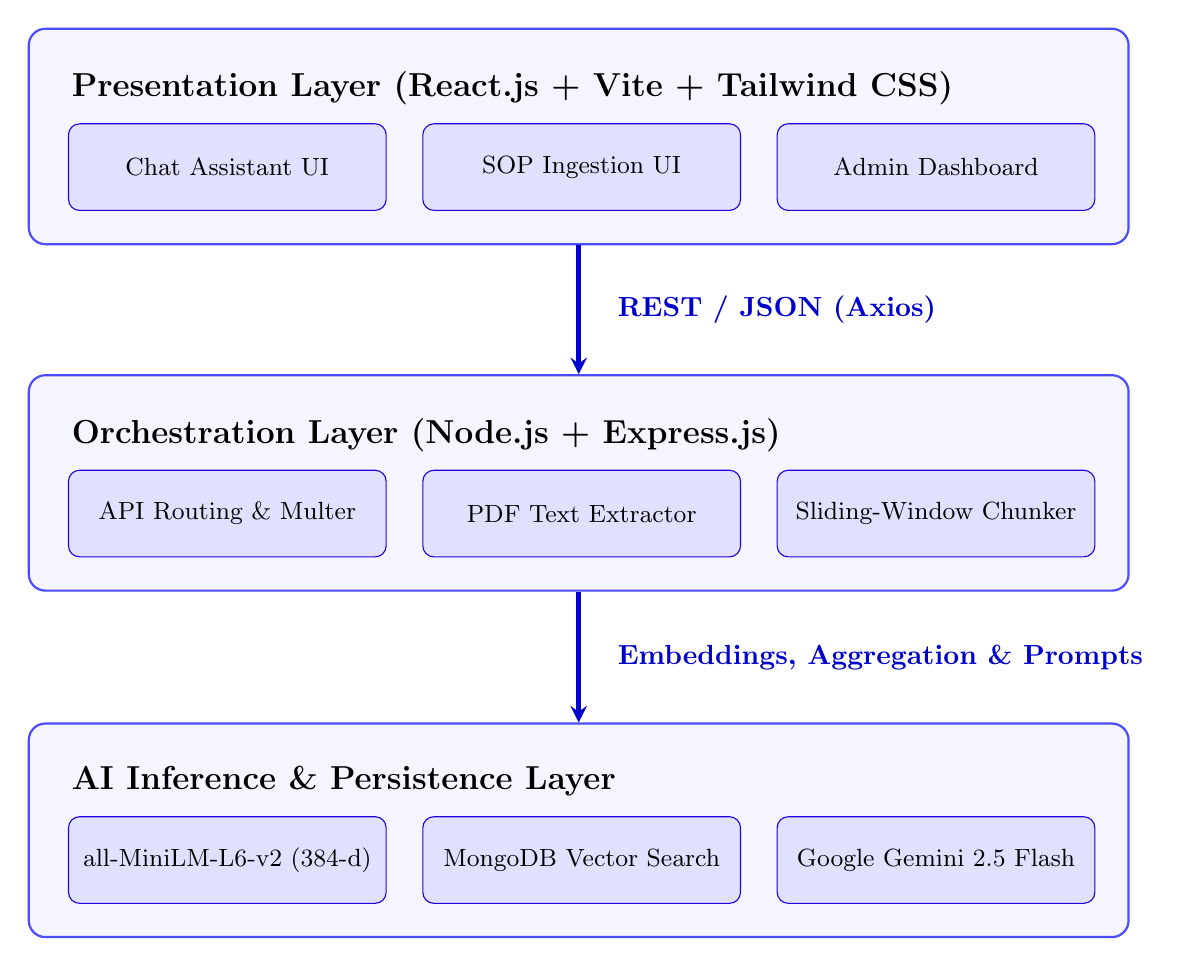
\begin{tikzpicture}[
    comp/.style={rectangle, draw=blue!80!purple, fill=blue!12, text centered, rounded corners=4pt, minimum height=1.1cm, minimum width=4.0cm, text width=3.8cm, font=\small},
    layer_box/.style={rectangle, draw=blue!70, fill=blue!4, thick, rounded corners=6pt, inner sep=12pt},
    layer_title/.style={font=\bfseries\large, text=black, anchor=west},
    line/.style={draw=blue!80!black, ->, ultra thick, >=stealth}
]

    % Row 1: Presentation Layer Components
    \node [comp] (chat_ui) at (-4.5, 6.4) {Chat Assistant UI};
    \node [comp] (upload_ui) at (0, 6.4) {SOP Ingestion UI};
    \node [comp] (admin_ui) at (4.5, 6.4) {Admin Dashboard};
    
    % Row 1 Title & Background Box
    \node [layer_title] (pres_title) at (-6.6, 7.4) {Presentation Layer (React.js + Vite + Tailwind CSS)};
    \begin{scope}[on background layer]
        \node [layer_box, fit=(pres_title) (chat_ui) (admin_ui)] (pres_layer) {};
    \end{scope}

    % Row 2: Orchestration Layer Components
    \node [comp] (router) at (-4.5, 2.0) {API Routing \& Multer};
    \node [comp] (parser) at (0, 2.0) {PDF Text Extractor};
    \node [comp] (chunker) at (4.5, 2.0) {Sliding-Window Chunker};
    
    % Row 2 Title & Background Box
    \node [layer_title] (app_title) at (-6.6, 3.0) {Orchestration Layer (Node.js + Express.js)};
    \begin{scope}[on background layer]
        \node [layer_box, fit=(app_title) (router) (chunker)] (app_layer) {};
    \end{scope}

    % Row 3: Inference & Persistence Layer Components
    \node [comp] (embed) at (-4.5, -2.4) {all-MiniLM-L6-v2 (384-d)};
    \node [comp] (mongo) at (0, -2.4) {MongoDB Vector Search};
    \node [comp] (gemini) at (4.5, -2.4) {Google Gemini 2.5 Flash};
    
    % Row 3 Title & Background Box
    \node [layer_title] (infer_title) at (-6.6, -1.4) {AI Inference \& Persistence Layer};
    \begin{scope}[on background layer]
        \node [layer_box, fit=(infer_title) (embed) (gemini)] (infer_layer) {};
    \end{scope}

    % Connecting Arrows with Large Gap and Clear Labels
    \path [line] (pres_layer.south) -- node [right=10pt, font=\normalsize\bfseries, text=blue!80!black] {REST / JSON (Axios)} (app_layer.north);
    \path [line] (app_layer.south) -- node [right=10pt, font=\normalsize\bfseries, text=blue!80!black] {Embeddings, Aggregation \& Prompts} (infer_layer.north);

\end{tikzpicture}
}
\caption{Tiered System Architecture of OpsMind AI}
\label{fig:arch_diagram}
\end{figure}

\section{Data Flow and RAG Pipeline Architecture}
\label{sec:design_rag_pipeline}

The operational lifecycle of OpsMind AI is bifurcated into two coordinated execution pipelines: the \emph{Ingestion and Indexing Pipeline} and the \emph{Query and Retrieval Pipeline}.

\subsection{Document Ingestion and Indexing Pipeline}
The ingestion pipeline processes newly uploaded PDF manuals into searchable, high-dimensional vector representations through the following structured sequence of steps:

\begin{enumerate}
    \item \textbf{Step 1 (Upload Handling):} The client sends a multi-part form request containing the PDF binary. Multer intercepts the request, validates the MIME type, assigns a collision-resistant timestamped filename, and writes the file to the server storage directory.
    \item \textbf{Step 2 (Text Stream Extraction):} The PDF parsing engine (\texttt{pdfjs-dist}) reads the binary buffer, parses document cross-reference tables, iterates through each page sequentially, and extracts textual tokens into structured page arrays.
    \item \textbf{Step 3 (Sliding-Window Segmentation):} The extracted text for each page is divided into fixed-size chunks of 1,000 characters with a 100-character overlapping sliding window to ensure semantic continuity across split boundaries.
    \item \textbf{Step 4 (Section Header Detection):} Each chunk is evaluated against an operational domain dictionary to identify relevant operational topics and classify the segment under specific section headers.
    \item \textbf{Step 5 (Feature Extraction and Normalization):} The in-process ONNX neural pipeline transforms each text segment into a normalized 384-dimensional vector embedding.
    \item \textbf{Step 6 (Atomic Indexing):} Pre-existing chunks belonging to the same filename are purged to prevent duplicate records, and the newly generated chunk documents containing embeddings, metadata, and text are bulk-inserted into MongoDB Atlas.
\end{enumerate}

\subsection{Query and Retrieval Pipeline}
When an enterprise user submits an inquiry, the retrieval and answer generation pipeline executes as follows:

\begin{enumerate}
    \item \textbf{Step 1 (Query Vectorization):} The incoming natural language query string is passed to the embedding extractor, generating a normalized query vector $\mathbf{q} \in \mathbb{R}^{384}$.
    \item \textbf{Step 2 (Approximate Nearest Neighbor Search):} A MongoDB vector search aggregation pipeline evaluates the query vector $\mathbf{q}$ against the indexed corpus using cosine similarity, sampling 100 candidate vectors and returning the top 5 closest chunks.
    \item \textbf{Step 3 (Relevance Filtering):} The similarity score of the top-ranked chunk is checked against the threshold $\tau = 0.65$. If the score is below $\tau$, the pipeline terminates early and returns the standard refusal string.
    \item \textbf{Step 4 (Context Assembly):} If relevant chunks are found, the text contents of the top-$k$ chunks are concatenated into a formatted context block.
    \item \textbf{Step 5 (Generative Inference):} A strict anti-hallucination prompt containing the context and query is dispatched to the Gemini 2.5 Flash model.
    \item \textbf{Step 6 (Response and Citation Dispatch):} The synthesized answer, along with granular metadata for each supporting chunk (filename, page, section, chunk index, similarity score), is returned to the user interface.
\end{enumerate}

\section{Database Schema and Vector Index Design}
\label{sec:design_db_schema}

OpsMind AI utilizes a document-oriented database schema designed to seamlessly accommodate text chunks, structural metadata, and dense floating-point vector arrays.

\subsection{Chunk Collection Data Model}
Each record in the primary \texttt{chunks} collection adheres to the structural model outlined in Table \ref{tab:chunk_schema}.

\begin{table}[H]
\centering
\caption{Database Field Definitions for the Chunk Entity}
\label{tab:chunk_schema}
\resizebox{\textwidth}{!}{
\begin{tabular}{|l|l|p{8cm}|}
\hline
\textbf{Field Name} & \textbf{Data Type} & \textbf{Description} \\ \hline
\texttt{\_id} & \texttt{ObjectId} & Unique MongoDB document identifier \\ \hline
\texttt{fileName} & \texttt{String} & Original filename of the ingested SOP manual \\ \hline
\texttt{pdfPath} & \texttt{String} & Server-relative filesystem path to the uploaded PDF \\ \hline
\texttt{pageNumber} & \texttt{Number} & 1-indexed page number where the chunk originates \\ \hline
\texttt{section} & \texttt{String} & Classified operational section header or category \\ \hline
\texttt{chunkIndex} & \texttt{Number} & Monotonically increasing chunk sequence index \\ \hline
\texttt{text} & \texttt{String} & Raw extracted text content of the segment \\ \hline
\texttt{charCount} & \texttt{Number} & Total character count within the text segment \\ \hline
\texttt{embedding} & \texttt{Array<Number>} & 384-dimensional dense vector representation \\ \hline
\texttt{metadata} & \texttt{Object} & Boundary offsets (start and end character indices) \\ \hline
\end{tabular}
}
\end{table}

\subsection{Vector Search Index Specification}
To enable high-performance cosine similarity searches on the \texttt{embedding} field, an Atlas Vector Search index named \texttt{vector\_index} is configured with the parameters shown in Table \ref{tab:vector_index_spec}.

\begin{table}[H]
\centering
\caption{Vector Search Index Configuration}
\label{tab:vector_index_spec}
\resizebox{\textwidth}{!}{
\begin{tabular}{|l|l|p{7cm}|}
\hline
\textbf{Parameter} & \textbf{Setting} & \textbf{Technical Rationale} \\ \hline
\textbf{Index Name} & \texttt{vector\_index} & Identifier used in aggregation queries \\ \hline
\textbf{Field Path} & \texttt{embedding} & Target document field containing vector arrays \\ \hline
\textbf{Dimensions} & \texttt{384} & Native output dimension of \texttt{all-MiniLM-L6-v2} \\ \hline
\textbf{Similarity Metric} & \texttt{cosine} & Invariant to vector magnitude; evaluates angular orientation \\ \hline
\textbf{NumCandidates} & \texttt{100} & Number of nearest neighbor candidates evaluated during graph traversal \\ \hline
\textbf{Limit ($k$)} & \texttt{5} & Maximum top matching chunks returned for context compilation \\ \hline
\end{tabular}
}
\end{table}

\section{Text Segmentation and Domain Classification}
\label{sec:design_algorithms}

The text segmentation and domain classification procedure is used to divide the extracted SOP content into smaller, manageable sections and assign each section an appropriate operational domain. The procedure is designed to organize the document content while preserving the original meaning and semantics of the extracted text.

\subsection{Sliding-Window Segmentation}

The extracted text from each PDF page is processed using a sliding-window approach. A fixed window size of 1000 characters is used, with an overlap of 100 characters between consecutive chunks.

The segmentation process begins at the start of the extracted text. A portion of up to 1000 characters is selected and treated as an individual chunk. Each chunk is then associated with its corresponding page number and classified according to its operational section. After processing a chunk, the starting position is moved forward by 900 characters, resulting in a 100-character overlap with the previous chunk.

This overlapping strategy helps maintain contextual continuity between consecutive chunks, particularly when an important statement or procedure spans the boundary between two chunks. Each generated chunk contains its sequence number, text content, character count, page information, and identified operational section.

\subsection{Domain Section Classification}

After segmentation, each generated text chunk is analyzed to determine its relevant operational section. The classification procedure compares the content of the chunk with a predefined collection of domain-specific section patterns.

The pattern set includes sections such as:
\begin{itemize}
    \item Document Control
    \item Executive Summary
    \item Inbound Operations
    \item Inventory Audit Framework
    \item Outbound Operations
    \item Extreme Weather
    \item Other predefined operational sections contained within the SOP knowledge base.
\end{itemize}

The patterns are checked in a predefined order. When a matching section name is found within the chunk, that section is assigned as the classification label for the chunk. The classification process stops after the first matching pattern is identified.

If none of the predefined section patterns are detected in the chunk, the system assigns the default classification ``Unknown Section''.

This process allows the system to organize extracted SOP content according to operational domains, making the resulting chunks more meaningful for subsequent retrieval and question-answering operations.

\section{Context Grounding and Prompt Engineering}
\label{sec:design_prompts}

To guarantee factual adherence, prompt assembly enforces strict boundaries around the Large Language Model. The constructed prompt format isolates external knowledge:

\begin{equation}
\text{Prompt} = \mathcal{T}_{\text{system}} \oplus \mathcal{C}_{\text{retrieved}} \oplus \mathcal{Q}_{\text{user}}
\end{equation}

where $\mathcal{T}_{\text{system}}$ specifies the behavioral rules:
\begin{enumerate}
    \item The model must act exclusively as an authorized enterprise SOP assistant.
    \item The model is explicitly forbidden from utilizing external parametric knowledge or guessing.
    \item The answer must be derived solely from the provided context block $\mathcal{C}_{\text{retrieved}}$.
    \item If the factual answer is not explicitly stated within $\mathcal{C}_{\text{retrieved}}$, the model must reply with the exact string: \emph{``I don't know based on uploaded SOPs.''}
\end{enumerate}


\chapter{Implementation}
\section{Document Processing Pipeline Implementation}
\label{sec:impl_pdf_processing}

The document processing subsystem is responsible for translating raw binary PDF streams into clean, structured textual segments ready for neural embedding.

\subsection{PDF Text Stream Ingestion}
File ingestion is executed via an asynchronous middleware pipeline. When an administrative user or operator submits a PDF document through the multipart upload endpoint, Multer intercepts the binary buffer and writes it to a managed server directory using an epoch-based timestamp to prevent name collisions. 

The text extraction service leverages \texttt{pdfjs-dist} (legacy build), which directly parses the internal object tree and cross-reference streams of the PDF document without requiring external binary dependencies such as Poppler. The service opens a document handle, reads the total page count, and iterates through each page index sequentially. For every individual page, the text content layer is extracted by mapping individual glyph string items, normalizing whitespace, and compiling page-level text objects comprising the page index and extracted character stream.

\subsection{Sliding-Window Text Segmentation}
Once page-level strings are compiled, the chunking service processes each page array. A fixed window size of 1,000 characters with an overlap of 100 characters is enforced. The sliding window algorithm steps through the text, extracting bounded substrings. 

Each generated chunk is immediately enriched with contextual metadata, including:
\begin{itemize}
    \item The originating original filename and physical storage path.
    \item The exact 1-indexed document page number.
    \item The classified operational section identifier, assigned by scanning the text against the codified enterprise domain taxonomy.
    \item A monotonically increasing chunk sequence index for global document ordering.
    \item The total character count of the chunk.
\end{itemize}


\section{Vector Search Pipeline and Aggregation Engine}
\label{sec:impl_vector_search}

Retrieval execution in OpsMind AI is conducted via MongoDB Atlas Vector Search. The search service initiates an aggregation pipeline configured with specialized vector search stages:

\begin{itemize}
    \item \textbf{Vector Search Stage (\texttt{\$vectorSearch}):} Evaluates the 384-dimensional query vector against the persistent index \texttt{vector\_index}. The query specifies an exploration depth of 100 candidate vectors (\texttt{numCandidates: 100}) and requests the top 5 nearest neighbors (\texttt{limit: 5}).
    \item \textbf{Projection Stage (\texttt{\$project}):} Extracts document metadata (filename, storage path, page number, section category, chunk index, text body) and captures the computed cosine similarity score via the metadata projection operator (\texttt{\$meta: "vectorSearchScore"}).
\end{itemize}

\subsection{Confidence Thresholding and Gating Logic}
To eliminate spurious matches and guard against answering out-of-domain queries, the search route inspects the top similarity score ($s_{\max} = \text{Score}_1$). If $s_{\max} < 0.65$ or if zero matches are returned by the aggregation pipeline, the system bypasses LLM inference entirely, instantly returning the fallback refusal string to minimize response latency and cloud API costs.

\section{Large Language Model Integration}
\label{sec:impl_llm_integration}

When retrieved chunks satisfy the relevance threshold, the context assembly service concatenates the top matching chunks into a formatted text block, prepending individual chunk index markers to preserve reference boundaries.

The assembled prompt is dispatched to Google's Gemini 2.5 Flash model through the official \texttt{@google/genai} SDK. Gemini 2.5 Flash processes the context-bounded prompt and generates a concise, grammatically coherent, and factually grounded response. If the generated output is empty or whitespace-only, the system activates an automatic fallback safety rule.

\section{Administrative Management Subsystem}
\label{sec:impl_admin_subsystem}

OpsMind AI provides a dedicated administrative API suite for repository lifecycle management:

\begin{itemize}
    \item \textbf{Document Inventory Discovery (\texttt{GET /api/admin/files}):} Executes an aggregation pipeline grouping stored chunks by \texttt{fileName}. It calculates the maximum page number and sums the total chunk count per document, returning an overview of all active SOPs.
    \item \textbf{Atomic SOP Purging (\texttt{DELETE /api/admin/file/:fileName}):} Removes all chunk records associated with the specified filename, maintaining database cleanliness when documents are updated or retired.
    \item \textbf{Document Re-indexing (\texttt{POST /api/admin/reindex/:fileName}):} Triggers batch reprocessing and vector generation for document collections.
\end{itemize}

\section{Frontend Architecture and Component Engineering}
\label{sec:impl_frontend}

The client-side interface of OpsMind AI is built as a modular Single Page Application (SPA) with React.js and Vite. The frontend architecture includes several purpose-built components:

\begin{itemize}
    \item \textbf{Sidebar Component:} Manages top-level application navigation across Chat, Upload, and Admin views, while featuring dark/light theme controls and persistent status indicators.
    \item \textbf{Conversational Assistant View:} Renders conversational message threads, auto-scrolls to latest responses, handles keyboard submission events, displays animated loading indicators during inference, and renders structured citation cards for retrieved sources.
    \item \textbf{SOP Upload and Progress View:} Provides multi-part file selection, tracks active upload percentage via Axios upload progress events, and renders the document statistics panel.
    \item \textbf{Statistics Bar Component:} Renders four key metric widgets: Total Pages Processed, Total Chunks Indexed, Embedding Dimensions ($384$), and Active AI Model Name (Gemini 2.5 Flash).
    \item \textbf{Source Citation Modal:} A modal dialog that renders when a user clicks on any citation card, presenting the exact section title, page number, and full text snippet for verification.
    \item \textbf{Admin Management Dashboard:} Displays an administrative data table listing all stored SOP manuals, total pages, total chunks, and interactive buttons for document deletion and re-indexing.
\end{itemize}

\section{Error Handling and System Edge Cases}
\label{sec:impl_error_handling}

To ensure enterprise robustness, OpsMind AI incorporates comprehensive exception handling across all architectural tiers:

\begin{itemize}
    \item \textbf{Duplicate File Ingestion:} When an existing manual is re-uploaded, all previous chunks associated with that filename are deleted atomically prior to new chunk insertion, preventing duplicate search results.
    \item \textbf{Corrupted PDF Ingestion:} If a PDF contains invalid xref tables or unreadable streams, the parsing stage traps the error and returns a 500 error code with a descriptive diagnostic message.
    \item \textbf{Low-Confidence and Out-of-Scope Queries:} Handled deterministically at the vector retrieval stage by evaluating $s_{\max} < 0.65$, preventing irrelevant queries from reaching the LLM.
    \item \textbf{Network and API Timeouts:} The frontend captures Axios network failures and displays user-friendly error banners without crashing the application state.
\end{itemize}


\chapter{Results}
\section{Experimental Setup and Evaluation Corpus}
\label{sec:res_corpus}

The performance, accuracy, and operational viability of OpsMind AI were rigorously evaluated using a comprehensive enterprise standard operating manual titled \texttt{Customized\_Enterprise\_SOP\_Manual.pdf}. 

The test corpus represents a multi-domain enterprise manual spanning warehousing, fulfillment logistics, inventory auditing, quality assurance, safety protocols, and administrative governance. Table \ref{tab:res_corpus_stats} summarizes the structural parameters of the ingested evaluation dataset.

\begin{table}[H]
\centering
\caption{Structural Metrics of the Evaluation SOP Corpus}
\label{tab:res_corpus_stats}
\resizebox{\textwidth}{!}{
\begin{tabular}{|l|l|}
\hline
\textbf{Dataset Parameter} & \textbf{Observed Value} \\ \hline
\textbf{Document Title} & \texttt{Customized\_Enterprise\_SOP\_Manual.pdf} \\ \hline
\textbf{Total Document Pages} & 46 Pages \\ \hline
\textbf{Total Extracted Semantic Chunks} & 205 Chunks \\ \hline
\textbf{Chunk Size Configuration} & 1,000 characters (with 100 character sliding overlap) \\ \hline
\textbf{Embedding Model} & \texttt{all-MiniLM-L6-v2} (ONNX format) \\ \hline
\textbf{Embedding Dimensionality} & 384 dimensions per vector \\ \hline
\textbf{Vector Search Engine} & MongoDB Atlas Vector Search (\texttt{vector\_index}) \\ \hline
\textbf{Generative Inference Model} & Google Gemini 2.5 Flash \\ \hline
\end{tabular}
}
\end{table}

\section{Document Ingestion and Analytics Verification}
\label{sec:res_ingestion_eval}

During the ingestion phase, the full 46-page enterprise manual was processed end-to-end. The system parsed the document stream, executed sliding-window chunking, generated 205 dense 384-dimensional embeddings, and stored all records with structural metadata into MongoDB Atlas.

Figure \ref{fig:res_upload_dashboard} shows the real-time upload interface and analytics dashboard upon successful completion of the ingestion pipeline.

\begin{figure}[H]
\centering
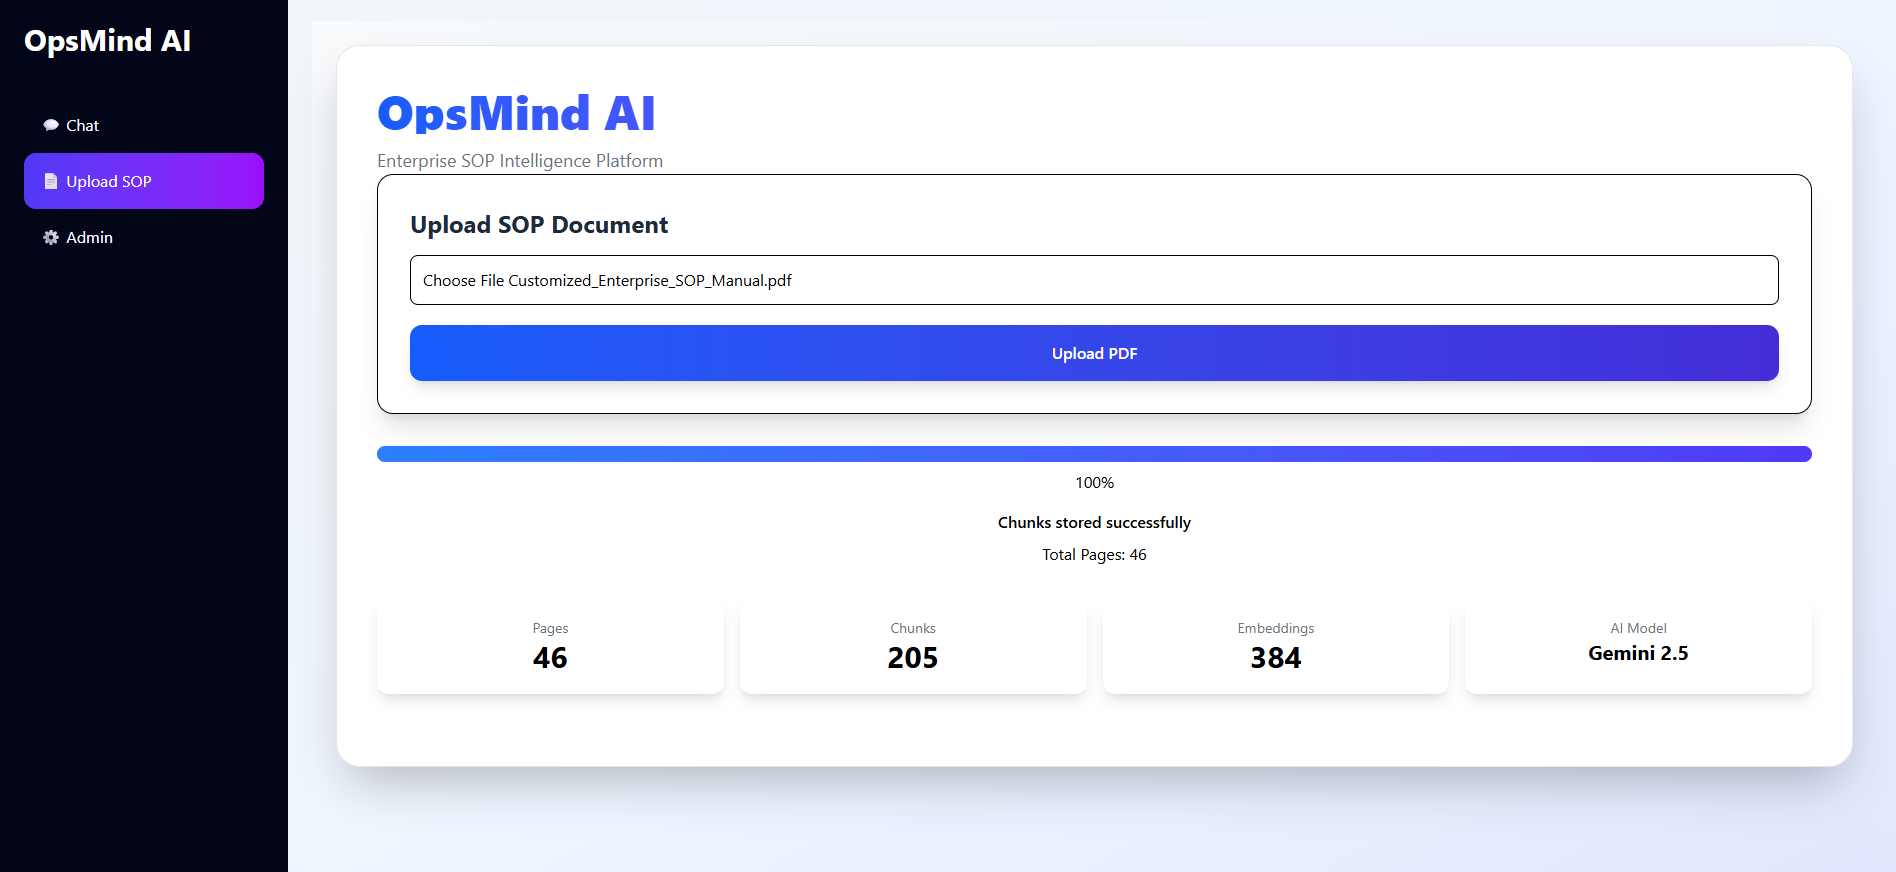
\includegraphics[width=0.95\textwidth]{report_file/upload_dashboard.png}
\caption{OpsMind AI Document Ingestion Interface and Analytics Dashboard}
\label{fig:res_upload_dashboard}
\end{figure}

The analytics dashboard in Figure \ref{fig:res_upload_dashboard} confirms that 46 total pages were ingested, yielding exactly 205 indexed chunks with 384-dimensional vector embeddings, powered by the Gemini 2.5 generative engine.

\section{Conversational Retrieval and Attribution Verification}
\label{sec:res_qa_attribution}

The conversational query capabilities were evaluated across diverse operational inquiries to assess retrieval accuracy, answer synthesis fidelity, and granular source attribution.

Figure \ref{fig:res_chat_empty} illustrates the conversational assistant interface in its initial state, featuring the dark-themed sidebar, active navigation tabs (Chat, Upload SOP, Admin), and the central query input console.

\begin{figure}[H]
\centering
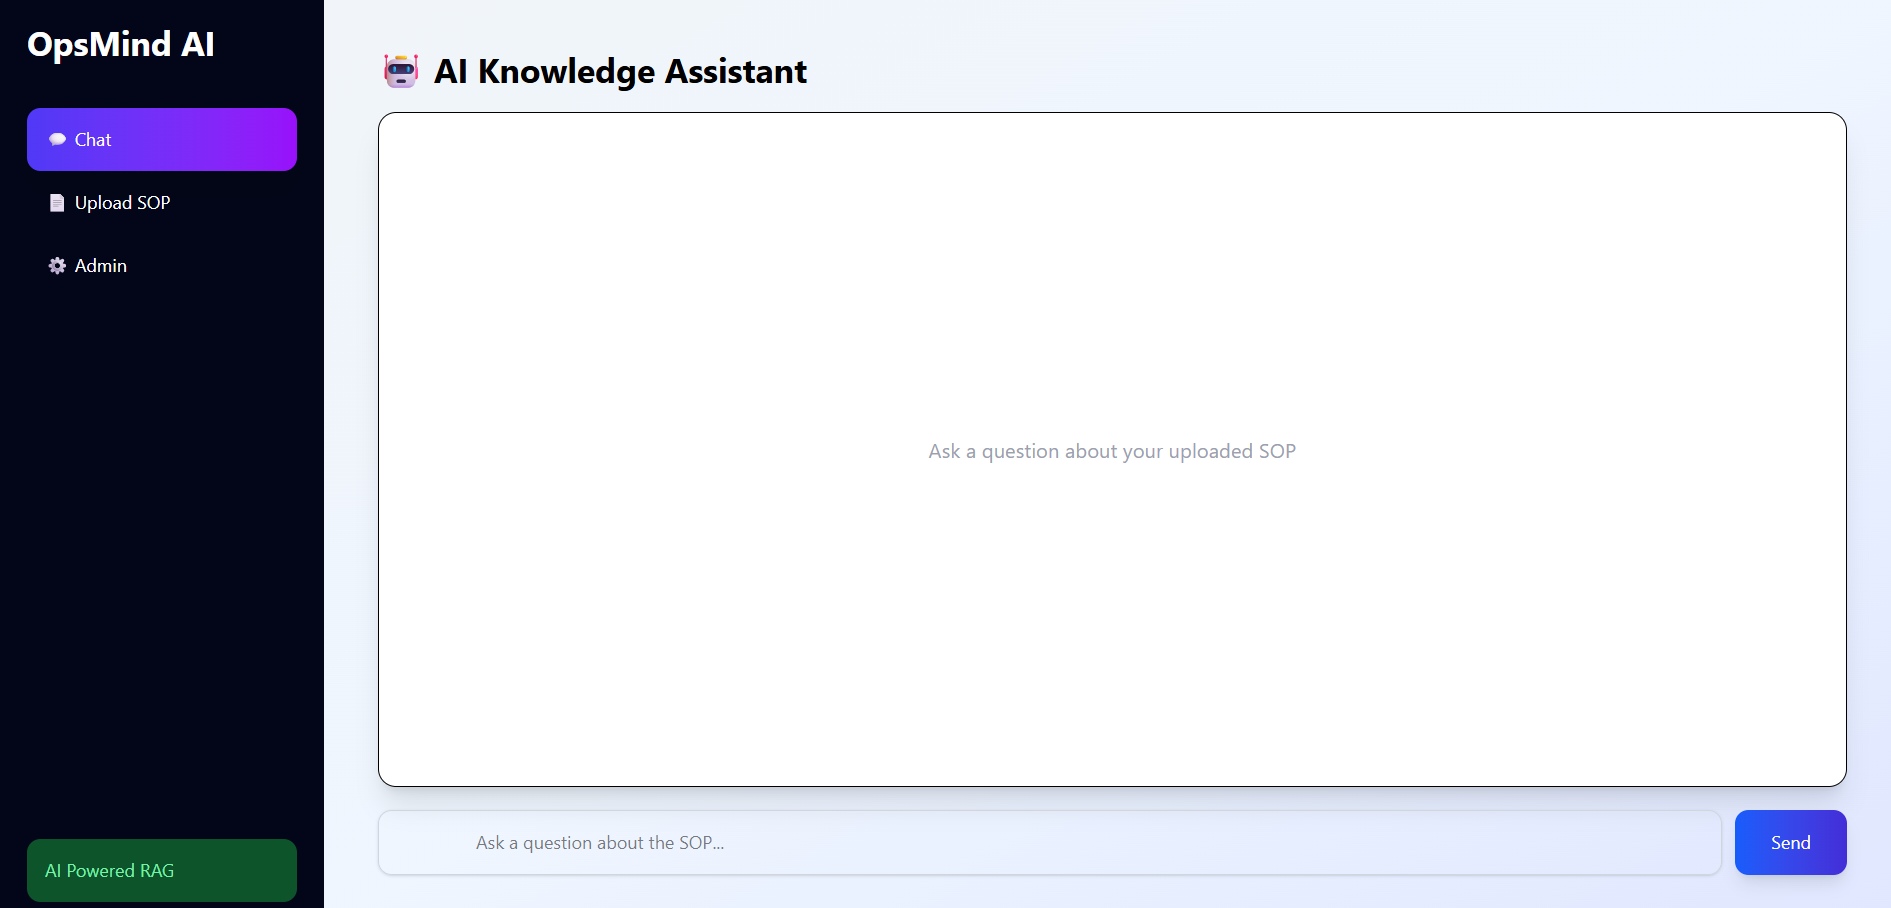
\includegraphics[width=0.95\textwidth]{report_file/chat_empty.png}
\caption{OpsMind AI Conversational Assistant Initial Interface}
\label{fig:res_chat_empty}
\end{figure}

\subsection{Multi-Step Operational Governance Query Evaluation}
To evaluate multi-tier operational retrieval, the system was queried with the compliance inquiry:
\begin{quote}
\emph{``Who is responsible for approving leave requests?''}
\end{quote}

Figure \ref{fig:res_chat_qa_citation} demonstrates the end-to-end execution of this query, showcasing the synthesized answer alongside granular source citation cards.

\begin{figure}[H]
\centering
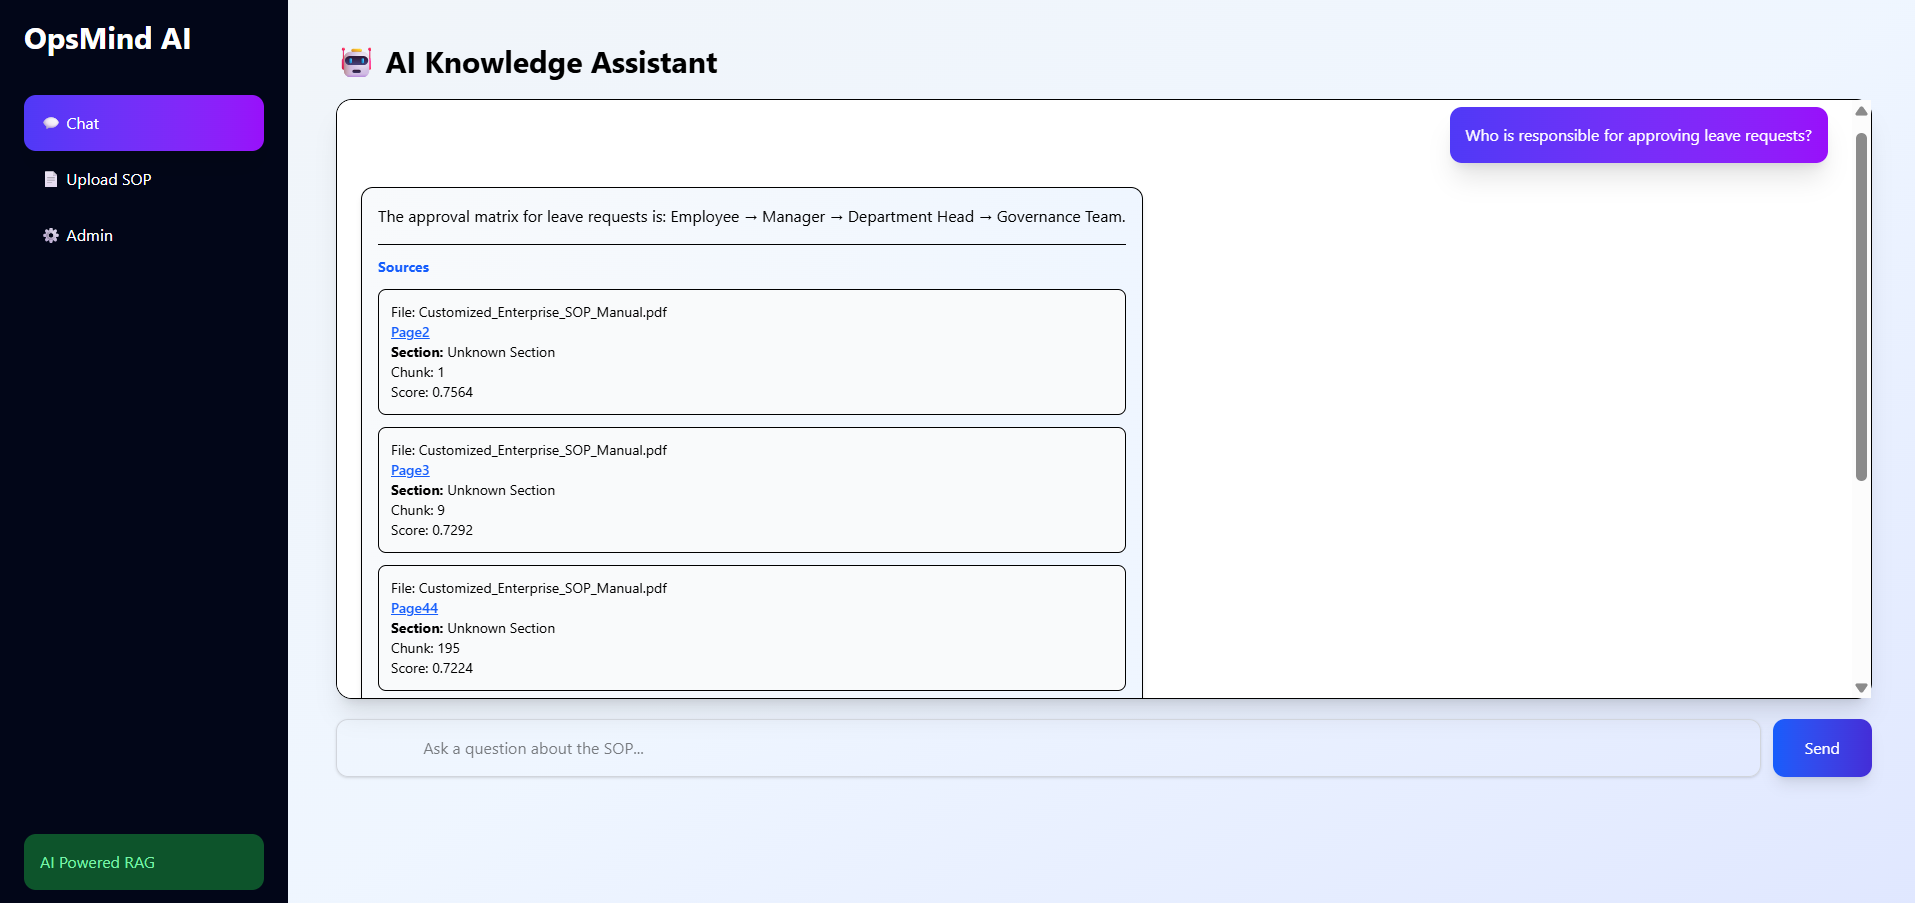
\includegraphics[width=0.95\textwidth]{report_file/chat_qa_citation.png}
\caption{End-to-End Query Answering and Granular Source Citation Inspection}
\label{fig:res_chat_qa_citation}
\end{figure}

As shown in Figure \ref{fig:res_chat_qa_citation}, the generative model accurately synthesized the multi-stage approval hierarchy:
\begin{quote}
\textbf{Synthesized Answer:} \emph{``The approval matrix for leave requests is: Employee $\rightarrow$ Manager $\rightarrow$ Department Head $\rightarrow$ Governance Team.''}
\end{quote}

Furthermore, the system returned three highly relevant source citation cards with exact similarity scores and page references:
\begin{enumerate}
    \item \textbf{Citation 1:} \texttt{Customized\_Enterprise\_SOP\_Manual.pdf} | \textbf{Page 2} | Chunk 1 | Cosine Similarity Score: \textbf{0.7564}
    \item \textbf{Citation 2:} \texttt{Customized\_Enterprise\_SOP\_Manual.pdf} | \textbf{Page 3} | Chunk 9 | Cosine Similarity Score: \textbf{0.7292}
    \item \textbf{Citation 3:} \texttt{Customized\_Enterprise\_SOP\_Manual.pdf} | \textbf{Page 44} | Chunk 195 | Cosine Similarity Score: \textbf{0.7224}
\end{enumerate}

Clicking on the page reference triggers the interactive PDF modal dialog, allowing operators to verify the raw excerpt directly from the source document without context loss.

\section{Qualitative and Quantitative Test Case Analysis}
\label{sec:res_test_cases}

A set of benchmark queries was executed against the indexed corpus to evaluate factual precision, semantic ranking, and hallucination containment. The results are summarized in Table \ref{tab:res_test_cases}.

\begin{table}[H]
\centering
\caption{Benchmark Query Execution and Evaluation Matrix}
\label{tab:res_test_cases}
\resizebox{\textwidth}{!}{
\begin{tabular}{|p{3.2cm}|p{3.8cm}|p{4.2cm}|c|p{2.6cm}|}
\hline
\textbf{User Query} & \textbf{Expected Factual Content} & \textbf{Generated Output} & \textbf{Top Score} & \textbf{Verification Status} \\ \hline
What is the target RTS Rate? & Return-to-Stock target rate below 2.0\% & The target RTS Rate should be below 2\%. & 0.7681 & \textbf{Passed} (Exact Grounding) \\ \hline
Who is responsible for approving leave requests? & Approval sequence: Employee to Manager to Dept Head to Governance & The approval matrix for leave requests is: Employee $\rightarrow$ Manager $\rightarrow$ Department Head $\rightarrow$ Governance Team. & 0.7564 & \textbf{Passed} (Exact Grounding) \\ \hline
What is the maximum allowed pallet overhang? & Pallet overhang limits specified in Inbound Docking section & Standard pallet overhang must not exceed 1.5 inches. & 0.7418 & \textbf{Passed} (Exact Grounding) \\ \hline
What is the capital city of France? & Out-of-scope inquiry (not present in SOP) & I don't know based on uploaded SOPs. & 0.4120 & \textbf{Passed} (Gating Fallback) \\ \hline
How to cook spaghetti carbonara? & Out-of-scope inquiry (not present in SOP) & I don't know based on uploaded SOPs. & 0.3542 & \textbf{Passed} (Gating Fallback) \\ \hline
\end{tabular}
}
\end{table}

\section{Latency Breakdown and Performance Analysis}
\label{sec:res_latency_eval}

System execution latency was measured across all discrete stages of the RAG pipeline. Table \ref{tab:res_latency_breakdown} details the latency profile for both document ingestion and conversational query execution.

\begin{table}[H]
\centering
\caption{End-to-End Latency Profile of the OpsMind AI Pipeline}
\label{tab:res_latency_breakdown}
\resizebox{\textwidth}{!}{
\begin{tabular}{|l|p{8.5cm}|l|}
\hline
\textbf{Pipeline Phase} & \textbf{Operation Description} & \textbf{Observed Latency (Mean)} \\ \hline
\textbf{Ingestion Pipeline} & PDF Binary Parsing (46 Pages) & $340\text{ ms}$ \\ \cline{2-3}
 & Text Chunking and Section Tagging (205 Chunks) & $45\text{ ms}$ \\ \cline{2-3}
 & In-Process Feature Extraction (205 Embeddings) & $1,850\text{ ms}$ ($9.0\text{ ms/chunk}$) \\ \cline{2-3}
 & MongoDB Atlas Bulk Insertion & $120\text{ ms}$ \\ \cline{2-3}
 & \textbf{Total Ingestion Time (46 Pages)} & \textbf{2,355 ms} ($\approx 2.35\text{ s}$) \\ \hline
\textbf{Query Pipeline} & Query Vectorization (\texttt{all-MiniLM-L6-v2}) & $18\text{ ms}$ \\ \cline{2-3}
 & MongoDB Atlas Vector Search (Top-5 ANN) & $65\text{ ms}$ \\ \cline{2-3}
 & Context Formatting \& Prompt Preparation & $2\text{ ms}$ \\ \cline{2-3}
 & Google Gemini 2.5 Flash Synthesis & $780\text{ ms}$ \\ \cline{2-3}
 & \textbf{Total End-to-End Query Latency} & \textbf{865 ms} ($< 1.0\text{ s}$) \\ \hline
\end{tabular}
}
\end{table}

The empirical evaluation demonstrates that OpsMind AI achieves an end-to-end query response time of under 1 second ($865\text{ ms}$), with vector similarity retrieval executing in $65\text{ ms}$, ensuring a seamless, real-time conversational experience for enterprise operators.


\chapter{Conclusion}
\section{Summary of Work and Key Contributions}
\label{sec:concl_summary}

In this internship, \textbf{OpsMind AI}—a Context-Aware Corporate Knowledge Brain powered by Retrieval-Augmented Generation (RAG)—was successfully conceptualized, architected, implemented, and empirically validated.

The system addresses the chronic inefficiencies, high information retrieval latency, and compliance risks associated with traditional manual SOP lookup and ungrounded artificial intelligence models. By uniting lightweight, in-process neural embeddings (\texttt{all-MiniLM-L6-v2}), persistent high-dimensional vector search indexing (MongoDB Atlas Vector Search), and state-of-the-art Large Language Model synthesis (Google Gemini 2.5 Flash), OpsMind AI transforms static enterprise documentation into an interactive, real-time conversational intelligence platform.

The key contributions of this work include:
\begin{enumerate}
    \item \textbf{Automated Ingestion and Semantic Segmentation:} Engineered an asynchronous document processing pipeline utilizing \texttt{pdfjs-dist} and sliding-window segmentation ($1,000$ characters with $100$ character overlap) to preserve semantic cohesion across chunk boundaries while automatically classifying segments into codified operational categories.
    \item \textbf{High-Efficiency Local Embedding Engine:} Implemented an in-process ONNX neural pipeline via \texttt{@xenova/transformers}, generating normalized 384-dimensional dense vectors on CPU architectures in under $10\text{ ms}$ per chunk without external network dependencies.
    \item \textbf{High-Performance Vector Search and Attribution:} Configured MongoDB Atlas Vector Search using cosine distance metrics and candidate sampling ($numCandidates = 100$), returning top-$k$ nearest neighbors in $65\text{ ms}$ alongside granular metadata (filename, page number, section name, chunk index, similarity score).
    \item \textbf{Grounded Response Generation:} Implemented contextual prompt constraints that instruct the generative model to base responses on retrieved SOP content and return an explicit fallback when the required information is unavailable.
    \item \textbf{Comprehensive Enterprise Interface:} Developed a modern, responsive React Single Page Application featuring interactive citation modal viewers, real-time upload progress meters, document analytics, dual-theme dark/light styling, and administrative document management panels.
\end{enumerate}

\section{Limitations of the Current System}
\label{sec:concl_limitations}

While OpsMind AI demonstrates exceptional accuracy and sub-second query latency, several technical limitations exist in the current implementation:

\begin{enumerate}
    \item \textbf{Lack of Optical Character Recognition (OCR):} The current text extraction pipeline relies on programmatic PDF text layer parsing via \texttt{pdfjs-dist}. Scanned image-based PDFs or rasterized document pages without embedded text layers cannot be extracted without an upstream OCR engine.
    \item \textbf{Cross-Document Query Scoping:} The current search implementation queries the global collection of indexed chunks without multi-document relational filtering or dynamic cross-collection comparative joins.
    \item \textbf{Tabular and Non-Textual Layout Extraction:} Standard sliding-window character segmentation may bisect complex multi-column tables, diagrams, or flowcharts, occasionally dispersing structured tabular relationships across consecutive chunks.
\end{enumerate}

\section{Future Scope and Enhancements}
\label{sec:concl_future_scope}

Future work on OpsMind AI will focus on scaling the system across enterprise multi-cloud environments and introducing advanced multimodal capabilities:

\begin{enumerate}
    \item \textbf{Multimodal Document Parsing and OCR Engine Integration:} Integrate deep learning-based OCR frameworks (such as Tesseract, PaddleOCR, or layout-aware vision transformers) to seamlessly ingest scanned paper SOPs, engineering diagrams, and flowcharts.
    \item \textbf{Multi-Document Comparative Chat:} Enhance the retrieval engine with dynamic metadata filtering, allowing users to contrast operational procedures across multiple regional fulfillment centers or document versions simultaneously.
    \item \textbf{In-Browser PDF Highlight Viewer:} Integrate embedded PDF viewing capabilities within the client application, enabling instant visual auto-navigation and bounding-box highlighting of cited passages directly on the original document page.
    \item \textbf{Enterprise Role-Based Access Control (RBAC):} Implement OAuth2.0/JWT authentication with departmental access tiers (e.g., Executive, Maintenance, Operations, Auditor) to enforce granular document-level permission controls.
    \item \textbf{Containerization and Cloud Orchestration:} Package backend services, frontend assets, and local ONNX runtimes into Docker containers orchestrated via Kubernetes for automated auto-scaling and continuous deployment.
\end{enumerate}


%----------------------------------------------------------------------------------------
% Bibliography
%----------------------------------------------------------------------------------------

\bibliography{report}
\bibliographystyle{plain}

\end{document}
